
\documentclass[letterpaper,12pt]{article}
\usepackage{threeparttable}
\usepackage{geometry}
\geometry{letterpaper,tmargin=1in,bmargin=1in,lmargin=1.25in,rmargin=1.25in}
\usepackage[format=hang,font=normalsize,labelfont=bf]{caption}
\usepackage{amsmath}
\usepackage{multirow}
\usepackage{array}
\usepackage{delarray}
\usepackage{amssymb}
\usepackage{listings}
\usepackage{amsthm}
\usepackage{lscape}
\usepackage{natbib}
\usepackage{setspace}
\usepackage{float,color}
\usepackage[pdftex]{graphicx}
\usepackage{mathrsfs}  
\usepackage{pdfsync}
\usepackage{verbatim}
\usepackage{placeins} \usepackage{geometry}
\usepackage{pdflscape}
\synctex=1
\usepackage{hyperref}
\hypersetup{colorlinks,linkcolor=red,urlcolor=blue,citecolor=red}
\usepackage{bm}
\usepackage{amssymb}


\theoremstyle{definition}
\newtheorem{theorem}{Theorem}
\newtheorem{acknowledgement}[theorem]{Acknowledgement}
\newtheorem{algorithm}[theorem]{Algorithm}
\newtheorem{axiom}[theorem]{Axiom}
\newtheorem{case}[theorem]{Case}
\newtheorem{claim}[theorem]{Claim}
\newtheorem{conclusion}[theorem]{Conclusion}
\newtheorem{condition}[theorem]{Condition}
\newtheorem{conjecture}[theorem]{Conjecture}
\newtheorem{corollary}[theorem]{Corollary}
\newtheorem{criterion}[theorem]{Criterion}
\newtheorem{definition}{Definition} % Number definitions on their own
\newtheorem{derivation}{Derivation} % Number derivations on their own
\newtheorem{example}[theorem]{Example}
\newtheorem*{exercise}{Exercise} % Number exercises on their own
\newtheorem{lemma}[theorem]{Lemma}
\newtheorem{notation}[theorem]{Notation}
\newtheorem{problem}[theorem]{Problem}
\newtheorem{proposition}{Proposition} % Number propositions on their own
\newtheorem{remark}[theorem]{Remark}
\newtheorem{solution}[theorem]{Solution}
\newtheorem{summary}[theorem]{Summary}
\bibliographystyle{aer}
\newcommand\ve{\varepsilon}
\renewcommand\theenumi{\roman{enumi}}

\title{Math 320 Homework 5.2}
\author{Chris Rytting}

\begin{document}
\maketitle
\subsection*{5.6}


Given $A = \{(-1,2),(0,4),(1,-6),(2,-16)\}$  we have
\[p(x) = \frac{\sum_{j=0}^3 \frac{w_j}{x-x_j}y_j}{\sum_{j=0}^3 \frac{w_j}{x-x_j}}= \frac{\frac{1}{-1}\frac{1}{-2}\frac{1}{-3}}{(x+1)}(2) + \frac{\frac{1}{1}\frac{1}{-1}\frac{1}{-2}}{(x)}(-4)+\frac{\frac{1}{2}\frac{1}{1}\frac{1}{-1}}{(x-1)}(-6)+ \frac{\frac{1}{3}\frac{1}{2}\frac{1}{1}}{(x-2)}(-16)\]
\[=\frac{\frac{1}{3(x+1)}-\frac{2}{x}+\frac{3}{x-1}-\frac{16}{6(x-2)}}{\frac{1}{-6(x+1)}+\frac{1}{2x}-\frac{1}{2(x-1)}+\frac{1}{6(x-2)}}=-\frac{29x^3}{56}+\frac{53x^2}{8}-\frac{93x}{4}+\frac{190}{7}\]


\subsection*{5.7}
Every time we evaluate
\[L_{n,j}(x) = \frac{w(x)}{(x-x_j)w_j}\]
we have to compute all $w_j \quad \forall n$ $n$ times. Therefore the naive lagrange interpolation has a temporal complexity of $O(n^2)$.

As for the barycentric weights given by
\[w_j = \prod_{k=0 , k\not=j}^n\frac{1}{(x_j-x_k)}\]
the computation thereof has a temporal complexity $O(n) \subset O(n^2)$.
After finding $w_j$, we have
\[p(x) = \frac{\sum_{j=0}^n \frac{w_j}{x-x_j}y_j}{\sum_{j=0}^n \frac{w_j}{x-x_j}}\]
which we will do $n $ times, so its temporal complexity is in $O(n)$ in the numerator. The same logic applies for the bottom, and then we divide the two sums so we have a temporal complexity of $O(2n+1) \subset O(n)$.
\subsection*{5.8}
See code.


\subsection*{5.9}
\begin{lstlisting}
import numpy as np
from matplotlib import pyplot as plt

def calculate_weights(j, xvector):
    wj = []
    for k in xrange(len(xvector)):
        if k != j:
            wj.append(1./(xvector[j]-xvector[k]))
    return np.prod(wj)

def polynomial(x, xvector,y,w):
    num = []
    den = []
    for j in xrange(len(x)):
        num.append(w[j]*y[j]/(xvector-x[j]))
        den.append(w[j]/(xvector-x[j]))
    num = sum(num)
    den = sum(den)
    return(num/den)

def f(x):
    return np.abs(x)

def problem8():
    x = [-1., 0., 1., 2.]
    y = [2., -4., -6., -16.]
    w = []
    for j in xrange(len(x)):
        w.append(calculate_weights(j,x))
    xvector = np.linspace(-1.1,2.1,100)
    a = polynomial(x,xvector,y,w)
    plt.plot(xvector, a)
    plt.plot(x,y)
    plt.show()

def problem9():
    v = [-1.5,1.5,-.1,1.1]
    pts = range(2,21)
    xvector = np.linspace(-1.1,2.1,100)
    norm = []
    for n in pts:
        x = np.linspace(-1,1,n+1)
        y = f(x)
        ax = plt.subplot(4,5,n-1)
        ax.axis(v)
        ax.plot(x,y)
        w = []
        for j in xrange(len(x)):
            w.append(calculate_weights(j,x))
        a = polynomial(x,xvector,y,w)
        ax.plot(xvector,a)
        ax.axes.get_xaxis().set_visible(False)
        ax.axes.get_yaxis().set_visible(False)
        norm.append(np.linalg.norm(y,ord = np.inf)-np.linalg.norm(a,ord=np.inf))
    plt.show()
    print norm
\end{lstlisting}
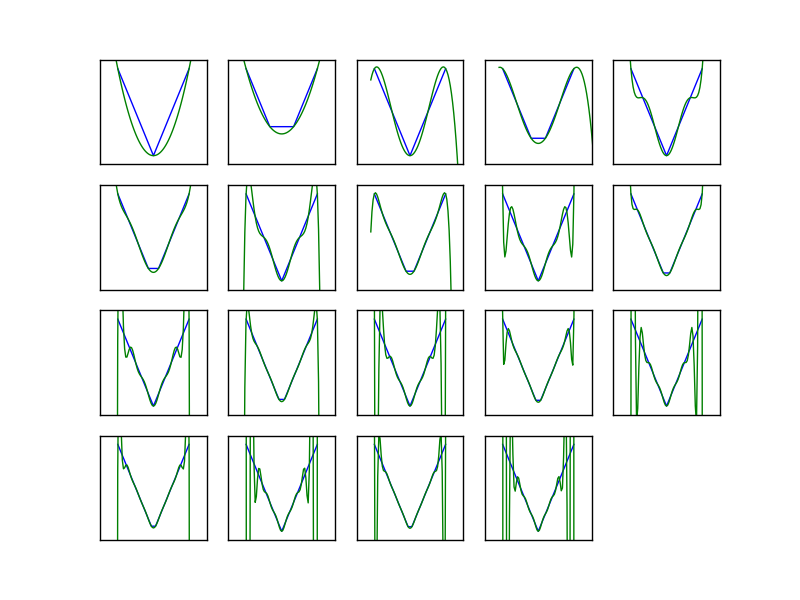
\includegraphics[scale=0.7]{figure1.png}\\
Finding the L infinity norm in python, we have that $n=3$ (4 points) is closest. 


\end{document}

